\documentclass{article}

\usepackage{graphicx}
\usepackage{parskip}
\usepackage{fullpage}
\usepackage{amsmath}
\usepackage{amsmath}
\usepackage{amsfonts}
\usepackage{amssymb}


\makeatletter
\newcommand*{\rom}[1]{\expandafter\@slowromancap\romannumeral #1@}
\makeatother

% Default fixed font does not support bold face
\DeclareFixedFont{\ttb}{T1}{txtt}{bx}{n}{12} % for bold
\DeclareFixedFont{\ttm}{T1}{txtt}{m}{n}{12}  % for normal

% Custom colors
\usepackage{color}
\definecolor{deepblue}{rgb}{0,0,0.5}
\definecolor{deepred}{rgb}{0.6,0,0}
\definecolor{deepgreen}{rgb}{0,0.5,0}

\usepackage{listings}

% Python style for highlighting
\newcommand\pythonstyle{\lstset{
language=Python,
basicstyle=\ttm,
otherkeywords={self},             % Add keywords here
keywordstyle=\ttb\color{deepblue},
emph={MyClass,__init__},          % Custom highlighting
emphstyle=\ttb\color{deepred},    % Custom highlighting style
stringstyle=\color{deepgreen},
frame=tb,                         % Any extra options here
showstringspaces=false            % 
}}


% Python environment
\lstnewenvironment{python}[1][]
{
\pythonstyle
\lstset{#1}
}
{}

% Python for external files
\newcommand\pythonexternal[2][]{{
\pythonstyle
\lstinputlisting[#1]{#2}}}

% Python for inline
\newcommand\pythoninline[1]{{\pythonstyle\lstinline!#1!}}

\begin{document}


\title{Personal Notes}
\author{Lucas Henry McConnell}

\maketitle
\tableofcontents

\section{General Physics}

\subsection{Bjorken x}
\emph{Bjorken x} is a Lorentz invariant used in QFT/RQM. One day when I learn more QFT I'll get a better handle on exactly what it is but until then I've gathered enough information to have a crude idea of how experimentalists use it.

Consider the Parton Model in which we treat the quarks within a colliding proton as free-particles that elastically scatter off each other. Now consider the Infinite Momentum Frame (IMF); this is the frame in which the proton has sufficiently high energy such that we can safely ignore the mass of the proton.\footnote{Bear in mind that we are also ignoring the mass of the quark and any transverse momentum to the proton's direction of motion.} Within the context of this model and this frame then, \textbf{\emph{Bjorken x} is the fraction of the proton's four-momentum carried by a given quark involved in a scatter process.}

\subsection{Bosons}
\emph{Bosons} are particles which have integer spin and which therefore are not constrained by the Pauli exclusion principle like the half-integer spin fermions. The energy distribution of bosons is described by Bose-Einstein statistics. The wavefunction which describes a collection of bosons must be symmetric with respect to the exchange of identical particles, while the wavefunction for a collection of fermions is antisymmetric.

At low temperatures, bosons can behave very differently to fermions because an unlimited number of them can collect into the same energy state. The collection into a single state is called condensation, or Bose-Einstein condensation. It is responsible for the phenomenon of superfluidity in liquid helium. Coupled particles can also act effectively as bosons. In the BCS Theory of superconductivity: coupled pairs of electrons act like bosons and condense into a state which demonstrates zero electrical resistance.

Bosons include photons and the characterisation of photons as particles with frequency-dependent energy given by the Planck relationship allowed Planck to apply Bose-Einstein statistics to explain the thermal radiation from a hot cavity.

\subsection{Bose-Einstein Condensation}
In 1924 Einstein pointed out that bosons could ``condense'' in unlimited numbers into a single ground state since they are governed by Bose-Einstein statistics and not constrained by the Pauli exclusion principle. Little notice was taken of this curious possibility until the anomalous behaviour of liquid helium at low temperatures was studied carefully.

When helium is cooled to a critical temperature of 2.17 K, a remarkable discontinuity in heat capacity occurs, the liquid density drops, and a fraction of the liquid becomes a zero viscosity ``superfluid''. Superfluidity arises from the fraction of helium atoms which have condensed to the lowest possible energy.

A condensation effect is also credited with producing superconductivity. In the BCS (Bardeen?Cooper?Schrieffer) Theory: pairs of electrons are coupled by lattice interactions, and the pairs (called Cooper pairs) act like bosons and can condense into a state of zero electrical resistance.

The conditions for achieving a Bose-Einstein condensate are quite extreme. The participating particles must be considered to be identical, and this is a condition that is difficult to achieve for whole atoms. The condition of indistinguishability requires that the deBroglie wavelengths of the particles overlap significantly. This requires extremely low temperatures so that the deBroglie wavelengths will be long, but also requires a fairly high particle density to narrow the gap between the particles.

Since the 1990s there has been a surge of research into Bose-Einstein condensation since it was discovered that Bose-Einstein condensates could be formed with ultra-cold atoms. The use of laser cooling and the trapping of ultra-cold atoms with magnetic traps has produced temperatures in the nanokelvin range. Cornell and Wieman along with Ketterle of MIT received the 2001 Nobel Prize in Physics "for the achievement of Bose-Einstein condensation in dilute gases of alkali atoms, and for early fundamental studies of the properties of the condensates". Cornell and Wieman led an active group at the University of Colorado, Boulder which has produced Bose-Einstein condensates with rubidium atoms.
\subsection{Control Region}
A control region is a region used to test our understanding of a background process by specifically selecting a region where a certain background is dominant.
\subsection{Dalitz Decay}
A Dalitz decay is a meson decay that involves two leptons in the final state, plus a photon. a double Dalitz decay has four leptons in the final state.
\subsection{Detector Acceptance vs. Detector Efficiency}
Let's consider the well known equation in particle physics:
$$ \frac{dN}{dt} = \sigma \mathcal{L}.$$
Integrating with respect to time we get:
$$N = \sigma \mathcal{L}_{inst.}.$$

In practice however things are no so simple. The equation should really be:
$$ N = A \varepsilon \sigma \mathcal{L}_{int.}$$.

Here $A$ is the detector acceptance (i.e. Did we build a big enough detector?), while $\epsilon$ is the detector efficiency (i.e. Did we build a good enough detector?).
\subsection{Drell-Yan Process}

The Drell-Yan process occurs in high energy hadron-hadron scattering. It takes place when a quark of a hadron and and antiquark of another hadron annhilate, creating a virtual photon or Z boson which then decays into a pair of oppositely-charged leptons. This is process was first suggested by Sidney Drell and Tung-Mow Yan in 1970 to decribe production of lepton-antilepton pairs in high-energy hadron collisions.

\centerline{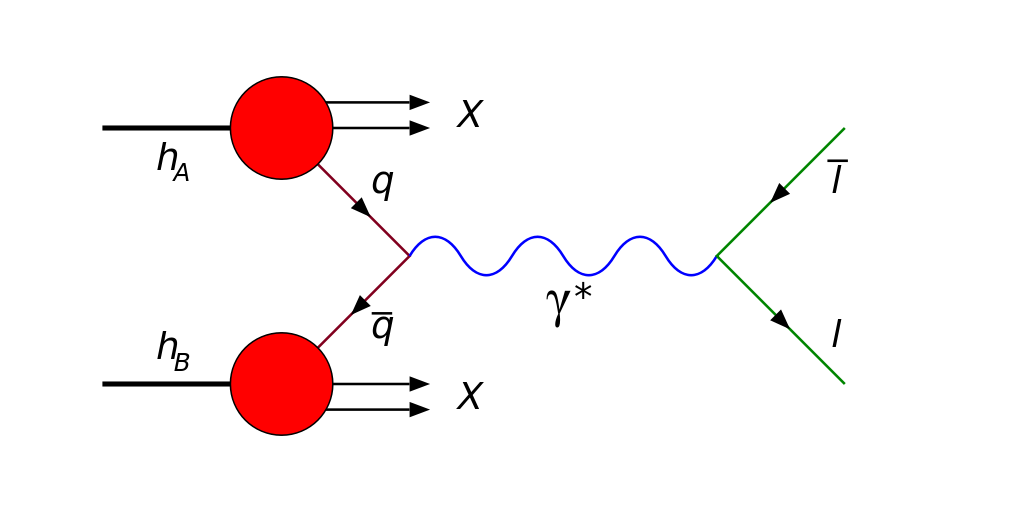
\includegraphics[scale=0.25]{1024px-Drell-Yan.png}}

\subsection{Elastic vs. Inelastic for proton-proton collisions}
Simply out an elastic proton-proton collision is : $p + p \longrightarrow p + p$.

While an inelastic collision is: $p + p \longrightarrow X$ (where X is anything but $p + p$).

\subsection{Fermions}
\emph{Fermions} are particles which have half-integer spin and therefore are constrained by the Pauli exclusion principle. Particles with integer spin are called bosons. Fermions include electrons, protons, and neutrons. The wavefunction which describes a collection of fermions must be antisymmetric with respect to the exchange of identical particles, while the wavefunction for a collection of bosons is symmetric.

The fact that electrons are fermions is foundational to the buildup of the periodic table of the elements since there can be only one electron for each state in an atom (only one electron for each possible set of quantum numbers). The fermionic nature of electrons also governs the behavior of electrons in a metal where at low temperatures all the low energy states are filled up to a level called the Fermi energy. This filling of states is described by Fermi-Dirac statistics.
\subsection{(The) Higgs Boson}
All the known forces in the universe are manifestations of four fundamental forces, the strong, electromagnetic, weak, and gravitational forces. But why four? Why not just one master force? Those who joined the quest for a single unified master force declared that the first step toward unification had been achieved with the discovery of the discovery of the W and Z particles, the intermediate vector bosons, in 1983. This brought experimental verification of particles whose prediction had already contributed to the Nobel prize awarded to Weinberg, Salam, and Glashow in 1979. Combining the weak and electromagnetic forces into a unified ``electroweak'' force, these great advances in both theory and experiment provide encouragement for moving on to the next step, the "grand unification" necessary to include the strong interaction.

While electroweak unification was hailed as a great step forward, there remained a major conceptual problem. If the weak and electromagnetic forces are part of the same electroweak force, why is it that the exchange particle for the electromagnetic interaction, the photon, is massless while the W and Z have masses more than 80 times that of a proton! The electromagnetic and weak forces certainly do not look the same in the present low temperature universe, so there must have been some kind of spontaneous symmetry breaking as the hot universe cooled enough that particle energies dropped below 100 GeV. The theories attribute the symmetry-breaking to a field called the Higgs field, and it requires a new boson, the Higgs boson, to mediate it.

\subsection{Jacobian Edge (from a comment made by Sahal)}
If you examine one leg of a two-particle decay and plot the $p_{t}$ spectrum:\\
\centerline{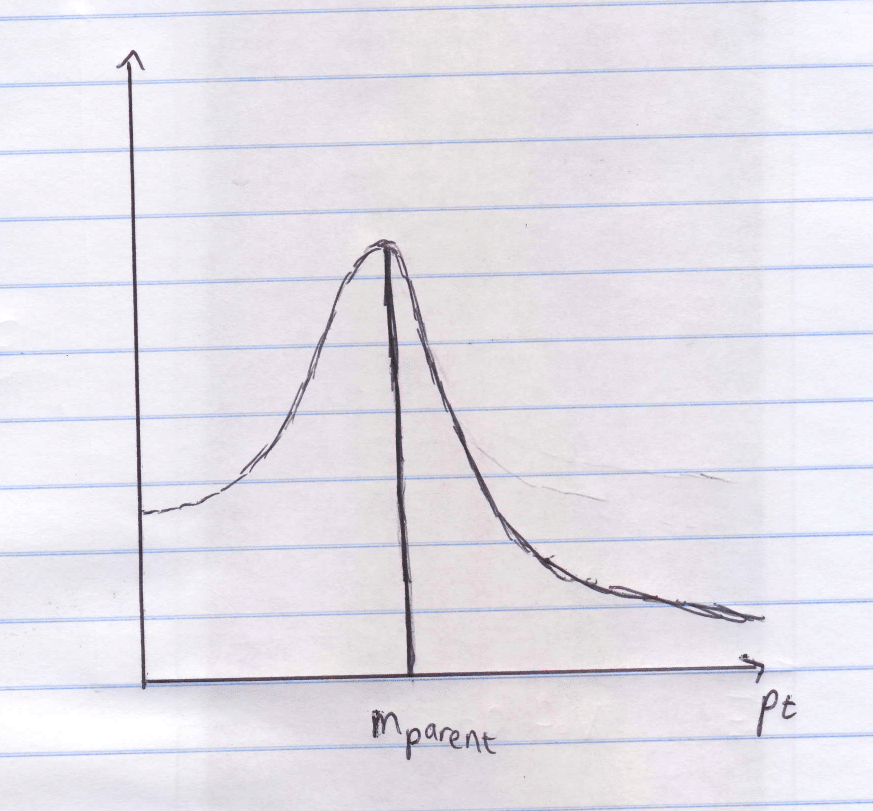
\includegraphics[scale=0.25]{jac_edge.png}}

The line from the tip of the peak is called the Jacobian Edge (or Shoulder) and it gives the mass of the parent particle.

\subsection{Jet Reconstruction}
In theoretical physics, a theorist will do QCD calculations in terms of the final state quarks and gluons. After hard scattering occurs, quarks and gluons will follow a branching process and then subsequently hadronise. The result is a collimated grouping of hadrons which is what is referred to as a QCD jet. In order to compare theoretical predictions with data, we need a way of mapping the partons resulting from a hard scatter to the actual final state hadrons observed in our detector. This mapping is what we refer to as the \emph{jet algorithm}. It is also necessary to have a structured way to assign four-momenta to particles within a jet, this is called the \emph{recombination scheme}. Taken together the jet algorithm and recombination scheme determine what we call the \emph{jet definition}. Such definitions are required to posses a variety of properties which I will not list here but suffice to say they must be ``well-behaved''. Please note that any jet algorithm worth using should have the property of being \emph{infrared safe}, i.e. it should avoid being dependent on the unknown, long-distance properties of QCD where perturbation theory breaks down.
\subsubsection{Seeded Fixed-Cone Algorithms (taken from Ryan's work)}
These algorithms attempt to reconstruct the jet by forming rigid cones centred on a point in $(\eta-\phi)$ space called the seed. Such algorithms are easy to implement but are not infrared safe.
\subsubsection{Sequential Recombination Jet Algorithms}
These are the most commonly applied class of jet algorithm. They revolve around having some measure of likely it is that two partons arose from the same QCD splitting. They then sequentially construct the jet by reconstructing the partons which are closer in this measure. The most basic form of this algorithm is the \emph{inclusive $k_{t}$ algorithm}. To use it first we define the following distances:
\begin{eqnarray}
d_{ij} & \equiv & min\left( p^{2}_{\mathbf{T},i};p^{2}_{\mathbf{T},j} \right) \frac{\Delta R_{ij}^{2}}{R^{2}} \\
d_{i \mathbf{B}} & \equiv & p_{\mathbf{T},i}^{2},
\end{eqnarray}
where \textbf{B} stands for Beam\footnote{As in the distance from the beam.}, $R$ is the radius of the jet and $\Delta R_{ij}^{2}  \equiv  \left( y_{i} - y_{j}\right)^{2} + \left( \phi_{i} - \phi_{j} \right) ^{2}$.
The algorithm then works as follows:
\begin{enumerate}
\item For all final state particles, determine all the distances $d_{ij}$ and $d_{i\mathbf{B}}$.
\item Find minimum distance.
\item If it is $d_{ij}$, then recombine particles $i$ and $j$ and go back to the first step.
\item Otherwise, declare particles $i$ to be a jet and remove from the list of particles. Back to step 1.
\item Terminate the algorithm when no particles remain.
\end{enumerate}
Actually, we can generalise the $k_{T}$ algorithm as follows:
\begin{eqnarray}
d_{ij} & \equiv & min\left( p^{2p}_{\mathbf{T},i};p^{2p}_{\mathbf{T},j} \right) \frac{\Delta R_{ij}^{2}}{R^{2}} \\
d_{i \mathbf{B}} & \equiv & p_{\mathbf{T},i}^{2p}.
\end{eqnarray}
The advantage of all sequential recombination jet algorithms over seeded fixed-cone algorithms is that they are all infrared safe. Some common values for $p$ are:
\begin{itemize}
\item $p = 1 \longrightarrow$ inclusive $k_{T}$ algorithm
\item $p = 0 \longrightarrow$ Cambridge/Aachen
\item $p = -1 \longrightarrow$ Anti-$k_{T}$ algorithm
\end{itemize}
In practise the Anti-$k_{T}$ algorithm is preferred over the inclusive $k_{T}$ algorithm as the computational time $T$ for the latter is $T= \mathcal{O}\left(N^{3}\right)$ while for the \emph{FastJet} implementation of the former $T = \mathcal{O}\left(N \ln {N}\right)$.
\subsection{Luminousity}
Luminousity can be informally thought of as: \emph{the number of particles passing down the beam line per unit time, per unit area.}

Luminousity ($\mathcal{L}$) is the ratio of the number of events detected (N) in a certain time (t) to the interaction cross-section ($\sigma$):

\begin{equation}
\mathcal{L} = \frac{1}{\sigma}\frac{dN}{dt}.
\end{equation}

It has dimensions of events per area.

Practically: $\mathcal{L}$ is dependant on the particle beam parameters, such as beam width and particle flow rate as well as the target propertie, such as target size and density.

A related quantity is the integrated luminousity ($\mathcal{L}_{int}$), which is the integral of the luminousity with respect to time:

\begin{equation}
\mathcal{L}_{int} = \int \mathcal{L} dt.
\end{equation}

All collider experiments aim to maximise their integrated luminousity, as the higher $\mathcal{L}_i{nt}$, the more data is available.
\subsection{On Shell and Off Shell}
In QFT, configurations that satisfy classical equations of motion are called on-shell, and those that do not are called off-shell.

Virtual particles are termed off-shell (mass-shell in this case) because they don't satisfy the Einstein energy-momentum relationship; real exchange particles do satisfy this relation and are termed on shell (mass-shell). In classical mechanics for instance, in the action formulation, extremal solutions to the variational principle are on shell and the Euler-Langrange equations give the on shell equations. Noether's theorem is also another on shell thereon.

\subsection{Pile-Up vs. Underlying Event}
\emph{Pile-Up} is defined as multiple semi-hard interactions from different $pp$ collisions in the same bunch crossing. On the other hand the \emph{Underlying Event} refers to the multiple semi-hard interactions in the same $pp$ collision.
\subsection{Rapidity and Pseudorapidity}
\subsubsection{Rapidity}
In theory: rapidity is an alternative to speed as a measure of rate of motion. Speed and rapidity are proportional a low speeds but rapidity becomes larger at high speeds and in particular the rapidity of light is infinite. A definition in this context is that \emph{rapidity is the hyperbolic angle differentiating two frame of reference in relative motion; with each frame being associated with distance and time coordinates}. Mathematically: $$ \varphi = \arctan \frac{| \mathbf{p}|}{E} = \frac{1}{2} \ln \frac{E + | \mathbf{p}|}{E - | \mathbf{p}|}. $$

Particle physicists use a modified definition of rapidity relative to the beam axis:
\begin{equation}
\label{rapidity}
y =  \frac{1}{2} \ln \frac{E+p_{z}}{E-p_{z}},
\end{equation}
where $p_{z}$ is the component of the three-momentum along the beam axis.
\subsubsection{Pseudorapidity}
\begin{figure}
\centering
\begin{minipage}{.5\textwidth}
  \centering
  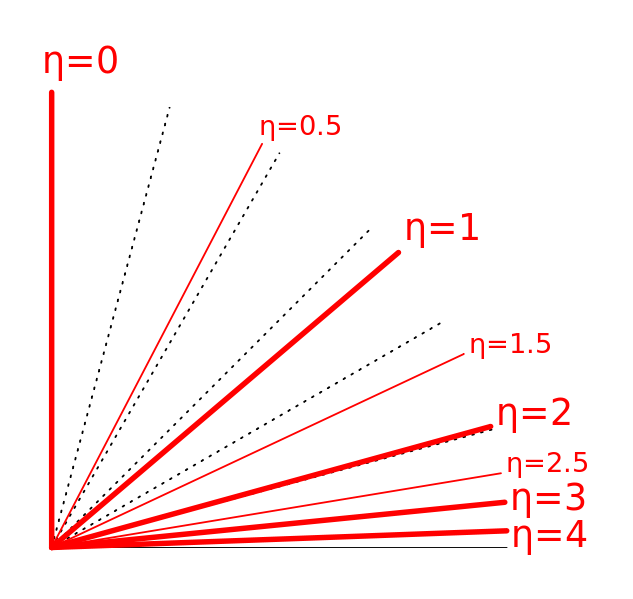
\includegraphics[width=.65\linewidth]{633px-Pseudorapidity_plot.png}
\end{minipage}%
\begin{minipage}{.5\textwidth}
  \centering
  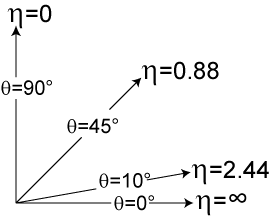
\includegraphics[width=.65\linewidth]{Pseudorapidity2.png}
\end{minipage}
\end{figure}
Pseudorapidity is a commonly used spatial angle of a particle relative to the beam axis. Mathematically: $$ \eta \equiv - \ln \left[ \tan \left( \frac{\theta}{2} \right) \right], $$ where $\theta$ is the angle between $\hat{\mathbf{p}}$ and the positive direction of the beam axis ($\hat{z}$).

Written in terms of momentum:
\begin{equation}
\label{pseudorapidity}
\eta = \frac{1}{2} \ln \left( \frac{|\mathbf{p}| + p_{z}}{|\mathbf{p}| - p_{z}} \right) = \tanh ^{-1} \left( \frac{p_{z}}{|\mathbf{p}|} \right),
\end{equation}
with $p_{z}$ being the three-momentum component along the beam axis.

Note that in the case of negligible mass equations \ref{rapidity} and \ref{pseudorapidity} are identical. In practise pseudorapidity is used for most physics objects except for jets in which neglecting the mass isn't a good assumption to take.

Rapidity and Pseudorapidity are preferred over the polar angle $\theta$ because, unlike $\theta$, differences in y and $ \eta $ are Lorentz invariant.
\subsection{Transverse Energy}
\label{trans_en}
\subsubsection{Overview}
Transverse momentum $p_{t}$, is the momentum of an object transverse to the beam. Transverse energy is defined as $E_{t} = \sqrt{m^{2} + p^{2}_{t}}$ for an object with invariant mass \emph{m} and transverse momentum $p_{t}$.

The initial longitudinal momentum in a parton collision is unknown, because the partons that make up a proton share the momentum. We do know however that the initial transverse momentum was zero. So we look for missing transverse momentum, defining $$p_{t}^{miss} = - \sum_{i} p_{t}(i)$$ for visible particles. Finding missing transverse momentum would indicate that new, unaccounted for particles has escaped the detector.

Confusingly, $$E_{t}^{miss} = - \sum_{i} p_{t}(i)$$ is commonly called missing transverse energy or MET. Missing transverse energy is equivalent to missing transverse momentum only if the missing particle(s) is(are) massless.
\subsubsection{Why do we use Transverse Energy instead of Longitudinal Energy? (notes from a discussion with Andrew and Sahal)}
Missing transverse energy is used to infer the presence of neutrinos. But why not use the missing longitudinal energy? After all even though before two protons collide in the LHC they have zero transverse momentum but they also have zero longitudinal momentum. There are two good reasons as to why transverse momentum is easier to work with than longitudinal momentum:
\begin{itemize}
\item There is a large bias for scatter products to be produced in the forward regions. Think back to your QCD studies with Peshier, the strong scattering there heavily favoured small scattering angles; it's the same thing here. Hence, the forward regions are heavily bombarded with scatter products and it is difficult to keep track of them all in order to reconstruct missing longitudinal energy $E_{long}^{miss}$. The more manageable numbers of scatter products in the transverse region make it more practical to work with $p_{T}$ and $E_{T}^{miss}$.
\item While the longitudinal energy of the two colliding protons is zero before collision, we do not know \emph{a priori} what the longitudinal component of the Bjorken x's of the scattering quarks will be. In contrast will do know that the transverse component of the Bjorken x's of the quarks is zero before they scatter making $E_{T}$ the ideal quantity to use.
\end{itemize}

\subsection{Transverse Mass}
Transverse mass $m_{T}$ is a useful quantity used by theorists. It is invariant under a Lorentz boost along the z-direction and is defined as : $m_{T}^{2} = m^{2} + p_{x}^{2} + p_{y}^{2}$.

However, experimentalists often encounter the situation in hadron physics where one particle in a two-particle decay cannot be directly measured and is only indicated by $E_{T}^{miss}$. Thus experimentalists more often use $m_{T}^{2} = \left( E_{T,1}^{2} + E_{T,2}^{2}\right)^{2} - \left(\textbf{p}_{T,1} + \textbf{p}_{T,2}\right)^{2}$. Where $E_{T}$ is defined as in \ref{trans_en}.

\subsection{Trigger Efficiency and the Resulting Bias (notes on discussion with Andrew)}
If you have a detector where the trigger efficiency as a function of $E_{t}$ looks like this:\\
\centerline{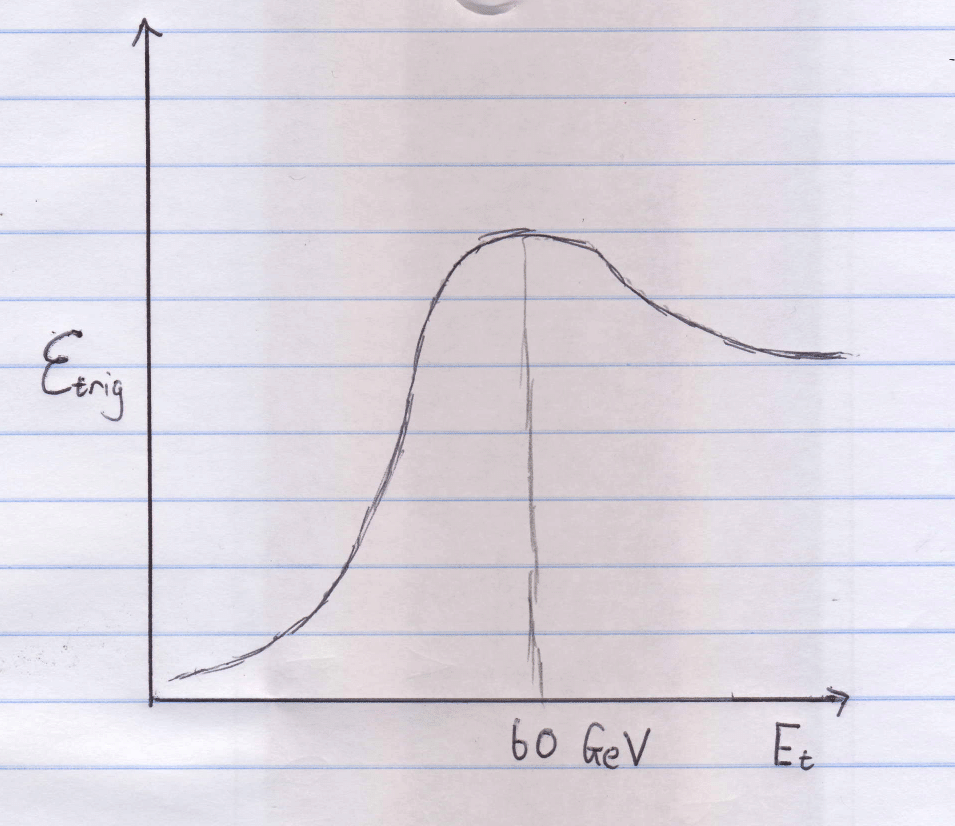
\includegraphics[scale=0.2]{trigger_eff.png}}
and it has a peak at say 60 GeV; then if you plot the $E_{t}$ spectrum for a photon pair, you'll see something like this:\\
\centerline{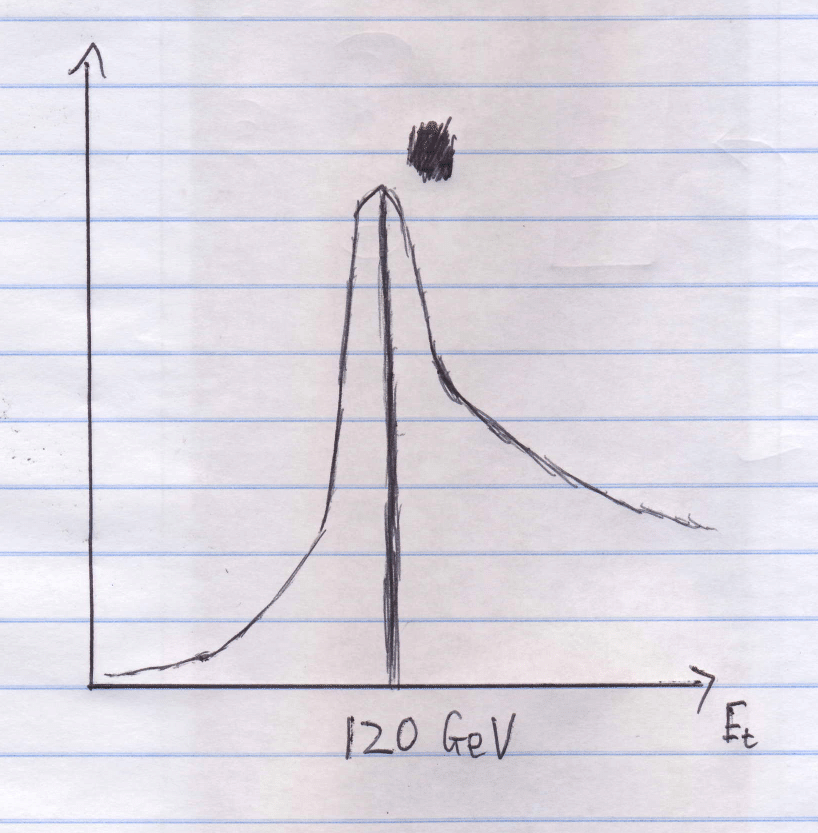
\includegraphics[scale=0.25]{trigg_bias.png}}
, since the trigger is biased towards detecting 60 GeV particles.
\subsection{Semi-leptonic Decay}
Semi-leptonic decay refers to a decay of a hadron through the weak interaction in which one lepton (and the corresponding neutrino) is produced in addition to one or more hadrons. An example of a semi-leptonic decay is $K^{0} \longrightarrow e^{-} + \bar{\nu}_{e} + \pi^{+}$.

This is to be contrasted with the purely hadronic decays, such as $K^{0} \longrightarrow \pi^{0} + \pi^{-}$, which are also mediated by the weak force.

Interestingly, semi-leptonic decays of neutral kaons have been used to study kaon oscillations.

\subsection{Simple calculation with cross-section and branching ratio (notes on discussion with Andrew)}
Let's say we have a case of $\mathcal{L} = 10 \ (fb)^{-1}$ and $\sigma(H^{++} = 100 \ fb$ knowing that a $H$ decays to a two $W$'s we then expect to see: $$ \mathcal{L}_{int} = \frac{N}{\sigma} \implies N = \sigma \mathcal{L}_{int}.$$ Plugging in some numbers then we might find: $$ N = 10 (fb)^{-1} \times 100 fb = 1000 \ events.$$ This is assuming that the branching ratio for a $H$ to decay to two $W's$ is 1 (i.e. certain).

Let's say we observed 0 ssWW events. How can we then set an upper bound on the cross-section $\sigma(H^{++})$? (This is still assuming a branching ratio $H \longrightarrow WW$ of 1.)

Well let's have a look at $N = 1$ event. If we have one event then: 
\begin{eqnarray}
N =& \sigma \mathcal{L}_{int}  \nonumber  \\
1 =& 100 \sigma & \implies \sigma = \frac{1}{10} \ fb \nonumber \\ 
\end{eqnarray}

Thus a decent upper bound on our $\sigma (H^{++})$ is: $\sigma \sim 0.1 \ fb$.
\subsection{Spin Classification}
One essential parameter for classification of particles is their ``spin'' or intrinsic angular momentum. Half-integer spin fermions are constrained by the Pauli exclusion principle whereas integer spin bosons are not. The electron is a fermion with electron spin 1/2.

The spin classification of particles determines the nature of the energy distribution in a collection of the particles. Particles of integer spin obey Bose-Einstein statistics, whereas those of half-integer spin behave according to Fermi-Dirac statistics.

\section{General Statistics}

\subsection{Overview}
Once you strip away all the bells and whistles, particle physics is essentially just statistics. An observation is an excess of events over an expected number of background events. The number of events in particle physics is given by:
$$ N = \mathcal{L} \times \sigma \times \varepsilon \times A. $$
Here $\mathcal{L}$ is the total integrated luminousity: the total number of $p-p$ collisions, at a particular energy, per area, that occurred during the period of data taking; $\sigma$ is the cross-section of the process. The value $\mathcal{L} \times \sigma$ will thus be the total number of $p-p$ collisions expected to have produced this process. The efficiency $\varepsilon$ and the acceptance $A$ are detector and reconstruction effects. These represent practical limitations and will necessarily lower the number of events. Some particle are not detected because they fall into inactive regions such as gaps in the detector or were absorbed by ``dead'' material. ``Dead'' material is all material that lies between detector components and does not make detections, e.g. the magnets and cryostats. This will lower the acceptance and hence $N$ overall.

To quantify the significance of the number of signal events (S) observed over the number of background events (B), one assumes a background-only hypothesis. This means the expected mean number of events is B with a standard deviation of $\sigma_{stat} = \sqrt{B}$, assuming Poissonian fluctuations. The p-value for an observation of $N = S + B$ events in a background-only hypothesis is:
$$p = 1 - \Phi \left(\frac{N-B}{\sqrt{B}}\right),$$
where $\Phi \left(\frac{N-B}{\sqrt{B}}\right)$ is the cumulative distribution function for the background-only normal distribution: effectively the area of the distribution from negative infinity to N.

The significance of this is the Z-value:
\begin{eqnarray}
Z &=& \Phi ^{-1} (1-p) \nonumber \\
 &=& \frac{N-B}{\sqrt{B}} \nonumber \\
 &=& \frac{S}{\sqrt{B}} \nonumber
\end{eqnarray}

This defines the significance of an excess of events above the expected background. For $ S << B$, this is a good but crude estimate for the significance. An approximate way of including systematic uncertainties in the background estimation is by taking the quadratic sum of the statistical and systematic uncertainties, $\sigma_{total}^{2} = \sigma_{stat}^{2} + \sigma_{sys}^{2}$. The significance then becomes:
$$ Z = \frac {S}{\sqrt{B+\sigma_{sys}^{2}}}.$$

In particle physics: a significance of $3 \sigma$ is defined as `evidence' of a signal, and a significance of $5 \sigma$ is defined as an `observation'. The events signifying the Higgs discovery were observed with a significance of 5.9 and 4.9 $\sigma$ by ATLAS and CMS respectively, with 10  fb$^{-1}$ of proton collision data.

\subsection{Signal-to-Background Ratio (from a discussion with Andrew)}
Andrew began by asking me: Why do we use Monte Carlo?
\begin{itemize}
\item To determine what our expect $s/b$ is.
\item To determine to what extent we understand our signal process.
\end{itemize}
Following from the answers given above we really want the signal-to-background ratio to be as large possible (within reason).

In order to observe and make references from data then, we should aim to have an excess of signal events over background events. Then the background can be ``cut away'' to make the signal more closely resemble the process we want to investigate. He sketched the famous picture of the Higgs discovery from the diphoton decay channel which I reproduce here:\\
\centerline{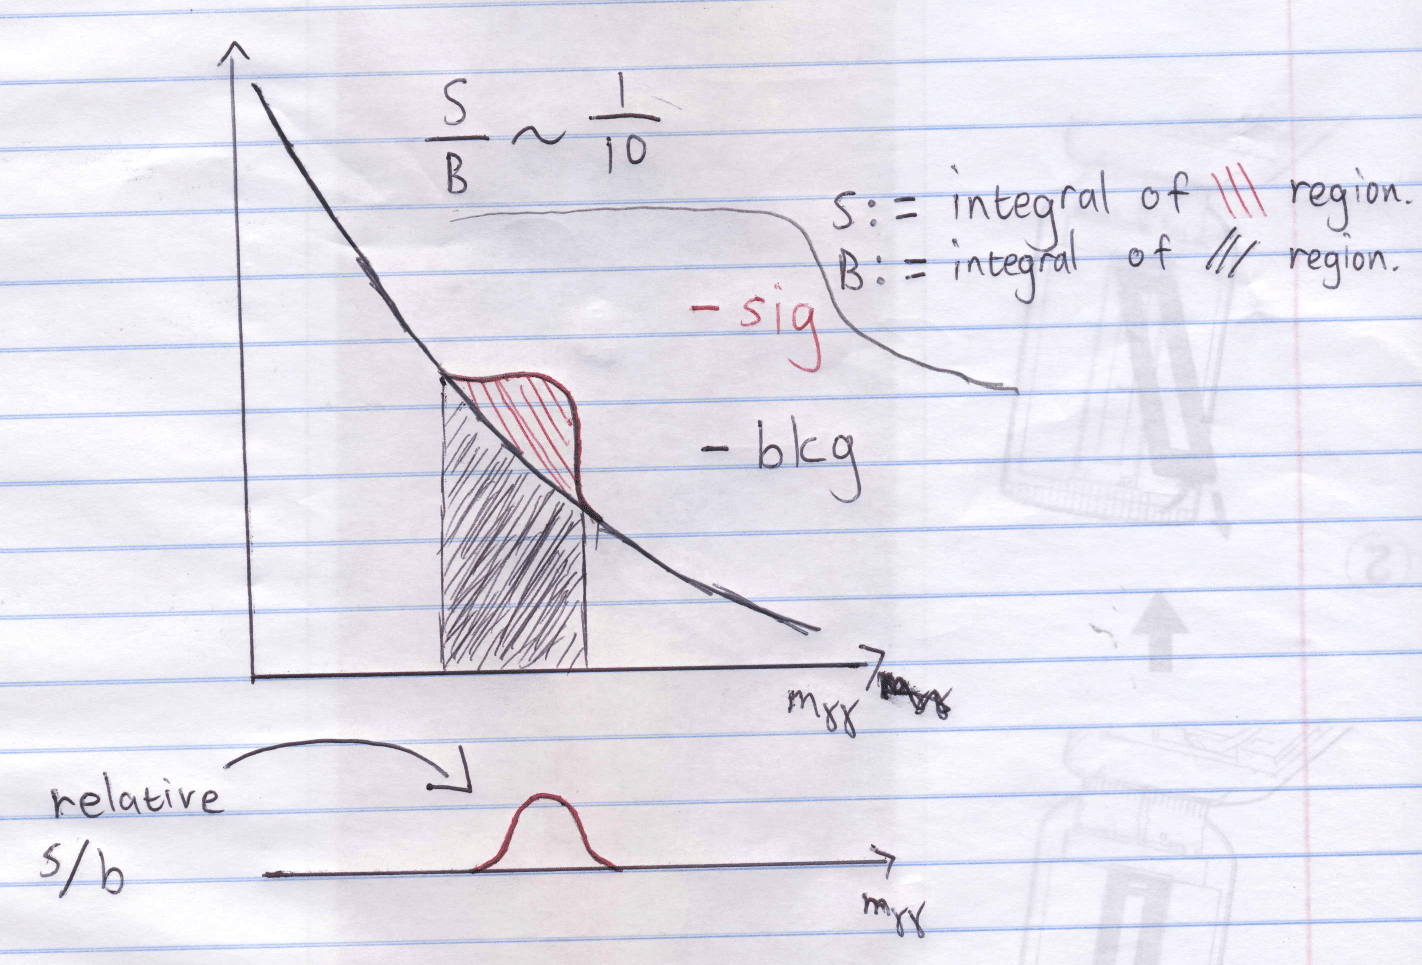
\includegraphics[scale=0.2]{higgs_disc.png}}
Here we are able to see the Higgs because of the clear excess of signal events over background events. This is despite there not being a good signal-to-background ratio here. This is because the number of actual events is also important and in practice using $s/\sqrt{s+b}$ is preferable to $s/b$ as it better takes this into account.

\subsection{What does sigma means in relation to confidence intervals?}
For example, in particle physics if a data set is said to meet a five sigma threshold, what does that actually mean?

It means that the results would occur by chance alone as rarely as a value sampled from a Gaussian distribution would be five standard deviations from the mean.

\section{General Computer Science}

\subsection{Some notes on OOP in Python}
In this code:
\begin{python}
class A(object):
	def __init__(self):
		self.x = 'Hello'
		
	def method_a(self,foo):
		print self.x + ' ' + foo
\end{python}
the \pythoninline{self} variable represents the instance of the object itself. Most OO languages pass this as a hidden parameter to the methods defined on an object; Python does not and you have to declare it explicitly. When you create an instance of the \pythoninline{A} class and call its methods, it will be passed automatically, as in
\begin{python}
a = A()	# We do not pass any argument to the __init__ method
a.method_a('Sailor')	# We only pass a single argument
\end{python}
The \pythoninline{__init__} method is roughly what represents a constructor in Python. When you call \pythoninline{A()} Python creates an object for you, and passes it as the first parameter to the \pythoninline{__init__} method. Any additional parameters (e.g. \pythoninline{A(24,'Hello')}) will also get passed as arguments -- in this case casuing an exception to be raised, since the constructor isn't expecting them.

\section{ATLAS Software}

\subsection{EventLoop}
EventLoop is the ATLAS approved way of reading run \rom{2} data (xAOD format and derivatives). EventLoop provides a framework to loop over input events and use approved tools in order to calibrate the physics objects.

\subsection{Flat Tuple}
A flat tuple (or nTuple) contains a root TTree object of values. It does not contain any other objects. Seems to be used as a simple way of working with data or MC without the usual overhead of all the individual objects otherwise present (like lepton or boson objects).

\subsection{QuickAna}
QuickAna is a framework that allows one to perform a quick analysis (as the name suggests). See ATLAS twiki for more info.

\subsection{TupleMaker}
TupleMaker makes an output file which has a copy of the objects and events we think we need in a simple, easily manipulated format without the overhead of EventLoop or QuickAna - mainly used for making quick plots.

\section{ssWW Analysis}

\subsection{Overlap Removal Order}
Since electron are formed from calorimeter deposits that are also reconstructed as jets, if a reconstructed jet and an electron lies within $\Delta R = 0.3$ of each other, the jet is discarded.

Since muons can radiate photons which can convert to electron-positron pairs, if a muon and an electron lie within $ \Delta R = 0.1$ of each other, the electron is discarded.

\subsection{Same-Sign vs. Opposite-Sign}
Why do we use the process of same-sign W-boson scattering to examine VBS instead of opposite-sign? The reasons lies with QCD. There is no leading-order gluon-gluon initial state present in the same-sign $W^{\pm}W^{\pm}$ scattering process, hence the $W^{\pm}W^{\pm}jj$ QCD contributions are very small.
\subsection{Truth Selection (Why do we need it?)}
The truth selection is needed to kill the fake leptons predicted by the MC as these are already accounted for by the data driven estimate.

The data-driven estimate is given by something like:\\
(Loose data + tight data) $\times$ fake-factor $-$ MC $\times$ fake-factor.

If the MC is accurately modelling the W+Jets background then the dd estimate should be close to zero. The truth selection makes the MC not include fake leptons in order to avoid ``double-counting''.

\subsection{Why are our jets forward?}
In general it's not a bad idea to think of s-channel processes as being isotropic or central. As a thought guide consider:\\

\centerline{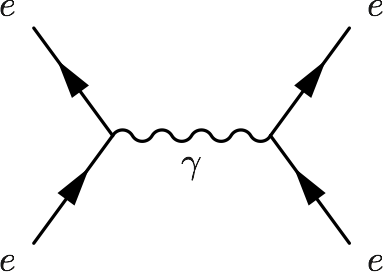
\includegraphics[scale=0.3]{s_channel.png}}

When the electron anti-electron pair annihilate they cease to exist and then reappear from the decay of the photon. This ``decay'' helps understand why s-channel processes are central. In contrast a t-channel process is more of a ``high speed glancing thing'' (to put it very roughly). So in a $p-p$ collision result in ssWW:\\

\centerline{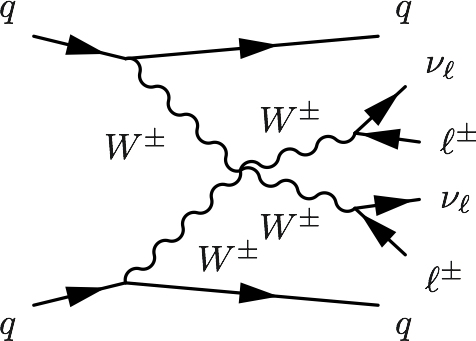
\includegraphics[scale=0.3]{signal.png}}

the resulting jets will ``inherit'' their ``forwardness'' from the original protons going down or up the beam line.

\end{document}